\chapter{Исследовательский раздел}

\section{Технические характеристики}

Тестирование проводилось на устройстве со следующими техническими характеристиками:

\begin{itemize}
	\item операционная система: Windows 10 Home;
	\item память: 8 GiB;
	\item процессор: AMD® Ryzen™ 3 3200u @ 2.6 GHz, 4 физических ядра;
	\item видеокарта: Radeon™ Vega 3 Graphics.
\end{itemize}

Тестирование проводилось на ноутбуке, включенном в сеть электропитания. Во время тестирования ноутбук был нагружен только встроенными приложениями окружения, а также непосредственно системой тестирования.

\section{Описание эксперимента}

Цель эксперимента заключается в выявлении зависимости времени обработки запросов к таблицам базы данных от использования индексирования. Эксперимент проводился на таблицах, содержащих информацию о винах и покупателях. В обеих таблицах хранятся 1000 записей.

Время выполнения поиска по первичному ключу в таблице вин показано на рисунке \ref{img:wineSearch}.

\includeimage
    {wineSearch}
    {f}
    {h}
    {1.0\textwidth}
    {Поиск по первичному ключу без использования индексирования}
    
Результаты выполнения запроса после создания индекса wine\_id\_index для первичного ключа таблицы вин, представленного на рисунке \ref{img:createWineIndex}, отображены на рисунке \ref{img:wineIndexSearch}.

\includeimage
    {createWineIndex}
    {f}
    {h}
    {1.0\textwidth}
    {Создания индекса для первичного ключа таблицы вин}
    
\includeimage
    {wineIndexSearch}
    {f}
    {h}
    {1.0\textwidth}
    {Поиск по первичному ключу c использованием индексирования}

Можно сделать вывод о том, что создание индекса не уменьшило время выполнения поиска по первичному ключу. Такой результат связан с автоматическим созданием индексов для первичных ключей.
   
Время выполнения поиска по внешнему ключу в таблице покупателей, объединенной с таблицей бонусных карт, показано на рисунке \ref{img:customerSearch}.

\includeimage
    {customerSearch}
    {f}
    {h}
    {1.0\textwidth}
    {Поиск по внешнему ключу без использования индексирования}
    
Результаты выполнения запроса после создания индекса bonus\_card\_id\_index для внешнего ключа таблицы покупателей (идентификатор бонусной карты), представленного на рисунке \ref{img:createCustomerIndex}, отображены на рисунке \ref{img:customerIndexSearch}.

\begin{figure}[H]
	\begin{center}
		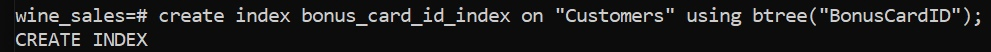
\includegraphics[scale=0.4]{inc/img/createCustomerIndex.jpg}
	\end{center}
	\captionsetup{justification=centering}
	\caption{Создания индекса для внешнего ключа таблицы покупателей}
	\label{img:createCustomerIndex}
\end{figure}

\begin{figure}[H]
	\begin{center}
		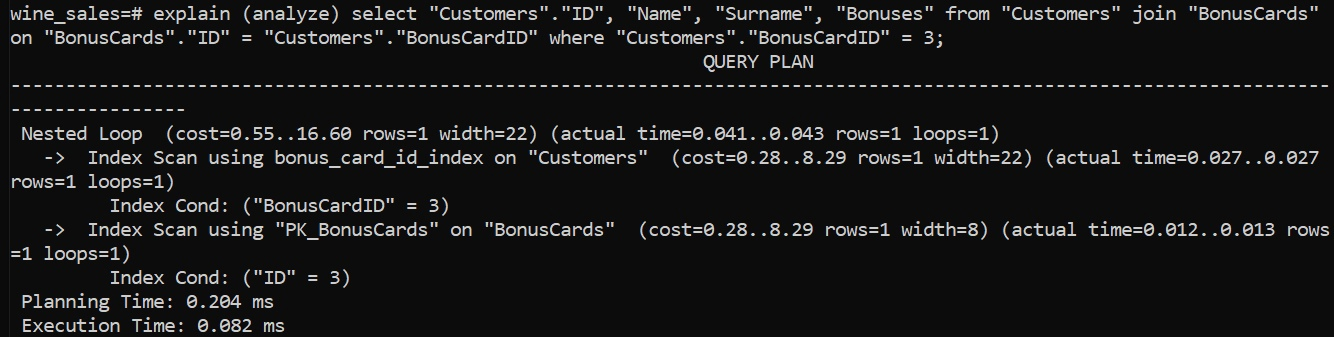
\includegraphics[scale=0.3]{inc/img/customerIndexSearch.jpg}
	\end{center}
	\captionsetup{justification=centering}
	\caption{Поиск по внешнему ключу c использованием индексирования}
	\label{img:customerIndexSearch}
\end{figure}

Можно сделать вывод о том, что создание индекса уменьшило время выполнения поиска по внешнему ключу в 3,8 раз. 

\section*{Вывод}

Проведенный эксперимент показал, что использование индексирования увеличивает скорость обработки запросов для внешних ключей. Создание индексов для первичных ключей не уменьшает время выполнения запросов, так как для первичных ключей индексы создаются автоматически.